\chapter{Geometría, información y ley del área de los agujeros negros}

\lectureoverview{El destino anunciado es la cosmología, pero el camino más corto empieza volviendo a la relatividad especial. Una métrica nos indica la geometría del espacio-tiempo, y la condición de tiempo propio nulo nos dice cómo se propaga la luz. Llevaremos esa regla a la geometría de Schwarzschild, distinguiremos el horizonte de la singularidad y luego preguntaremos qué ocurre con la información cuando un agujero negro se evapora. La respuesta empieza con la entropía ordinaria y termina con el argumento de Bekenstein basado en un bit: un agujero negro almacena información en unidades de área del horizonte, no de volumen.}

Susskind aplaza brevemente el balance prometido de los éxitos y fracasos de la teoría de cuerdas. Dice que es tarde y que resulta más útil abordar el contenido que hacer un balance. El contenido de esta noche es la geometría y la termodinámica mínimas necesarias para plantear el problema de la información de los agujeros negros.

\section{Una regla para la luz}

La relatividad especial trata el espacio y el tiempo como un único objeto geométrico. Para sucesos próximos separados por \(dt,dx,dy,dz\), Susskind adopta la convención de signos mayormente negativa y escribe
\begin{equation}
d\tau^2=dt^2-\frac{1}{c^2}\left(dx^2+dy^2+dz^2\right).
\end{equation}
Los signos opuestos de las partes temporal y espacial distinguen la geometría de Minkowski de la geometría euclidiana cuatridimensional. El factor \(1/c^2\) solo permite compatibilizar las unidades; si medimos el tiempo y la distancia de manera compatible, podemos fijar \(c=1\).

Para una separación temporal \(d\tau^2>0\), y \(d\tau\) es el tiempo propio registrado por un reloj que sigue la trayectoria. En cambio, las separaciones espaciales cumplen \(d\tau^2<0\). El caso que necesitamos esta noche está justo entre ambas. Un rayo de luz sigue una trayectoria \emph{nula},
\begin{equation}
d\tau^2=0.
\end{equation}
Si restringimos primero el movimiento al eje \(x\), obtenemos
\begin{align}
0&=dt^2-\frac{dx^2}{c^2},\\
c\,dt&=\pm dx,\\
\frac{dx}{dt}&=\pm c.
\end{align}
Los signos describen rayos que se propagan hacia la derecha y hacia la izquierda. El valor numérico asignado a \(c\) cambia al sustituir los centímetros por metros o kilómetros; la afirmación invariante no es un número, sino la condición de nulidad.

La relatividad general complica la métrica, pero no esta regla. Con coordenadas \(x^\mu\), \(\mu=0,1,2,3\),
\begin{equation}
ds^2=g_{\mu\nu}(x)\,dx^\mu dx^\nu,
\end{equation}
donde se suman los índices repetidos y los coeficientes pueden variar de un punto a otro. Para hallar las direcciones localmente permitidas para la luz, igualamos a cero esta forma cuadrática.

\section{Coordenadas esféricas y métrica de Schwarzschild}

Un agujero negro no rotatorio tiene simetría esférica, así que las coordenadas cartesianas ocultan la estructura útil. Sea \(r\) la distancia radial y sean \(\theta,\phi\) las coordenadas que indican una dirección sobre una esfera unitaria. Su elemento de línea es
\begin{equation}
d\Omega^2=d\theta^2+\sin^2\theta\,d\phi^2.
\end{equation}
Por tanto, sobre una esfera de radio \(r\), los desplazamientos angulares contribuyen con \(r^2d\Omega^2\). El espacio-tiempo plano en coordenadas esféricas es
\begin{equation}
d\tau^2=dt^2-\left(dr^2+r^2d\Omega^2\right),
\qquad (c=1).
\end{equation}

Susskind no deriva la solución del agujero negro a partir de las ecuaciones de Einstein. La escribe y nos pide que la examinemos. La pizarra hace explícita la comparación que se propone.

\begin{figure}[htbp]
\centering
\includegraphics[width=0.86\textwidth]{lecture_02_figure_02.png}
\caption{El espacio-tiempo esférico plano aparece sobre la deformación de Schwarzschild. Se ven juntos el factor repetido \(1-2GM/(c^2r)=1-R_s/r\) y el esquema radial.}
\lectureframe{00:19:12.520}
\end{figure}

Para un agujero negro de masa \(M\), definimos el radio de Schwarzschild
\begin{equation}
R_s=\frac{2GM}{c^2}.
\end{equation}
El elemento de línea exterior es
\begin{equation}
d\tau^2=\left(1-\frac{R_s}{r}\right)dt^2
-\frac{dr^2/c^2}{1-R_s/r}
-\frac{r^2}{c^2}d\Omega^2.
\label{eq:schwarzschild-explicit-c}
\end{equation}
De forma equivalente, al fijar \(c=1\),
\begin{equation}
ds^2=\left(1-\frac{2GM}{r}\right)dt^2
-\frac{dr^2}{1-2GM/r}-r^2d\Omega^2.
\label{eq:schwarzschild}
\end{equation}
A grandes distancias, \(R_s/r\ll1\), y se recupera la métrica esférica plana. Esta comprobación asintótica importa más que memorizar la fórmula, aunque Susskind recomienda esto último como tema de conversación para fiestas.

\editorialnote{La pizarra alterna entre \(d\tau^2\) y \(ds^2\), y no muestra de forma coherente todos los factores de \(c\). La ecuación~\eqref{eq:schwarzschild-explicit-c} sigue la convención de la coordenada temporal usada en la clase, en la que \(t\) tiene unidades de tiempo. La forma estándar con \(x^0=ct\) es algebraicamente equivalente.}

\subsection{El horizonte no es la singularidad}

Hay dos radios que parecen sospechosos en estas coordenadas. En \(r=R_s=2GM\), usando unidades naturales, el coeficiente de \(dt^2\) se anula y el de \(dr^2\) diverge. En \(r=0\), la propia curvatura se vuelve singular. No se trata de dos versiones del mismo suceso:
\begin{equation}
\begin{aligned}
r=R_s &:\quad \text{horizon},\\
r=0 &:\quad \text{curvature singularity}.
\end{aligned}
\end{equation}

Las fuerzas de marea establecen la distinción física. El campo gravitatorio varía a lo largo de un cuerpo extenso: puede tirar con más fuerza de los pies que de la cabeza, estirando el cuerpo mientras comprime las direcciones transversales. En el horizonte, esas fuerzas de marea son finitas y, en el horizonte de un agujero negro suficientemente masivo, pueden ser muy pequeñas. Allí no tiene por qué ocurrir nada catastrófico a nivel local. En cambio, en \(r=0\) las fuerzas de marea divergen. Los coeficientes alarmantes en \(r=R_s\) indican un defecto de las coordenadas de Schwarzschild; la singularidad en \(r=0\) es física.

\editorialnote{La finitud de la curvatura en \(r=R_s\) puede comprobarse mediante el escalar de Kretschmann \(R_{\mu\nu\rho\sigma}R^{\mu\nu\rho\sigma}=48G^2M^2/(c^4r^6)\), que es finito en el horizonte y solo diverge cuando \(r\to0\). Este invariante no se escribió en la clase, pero precisa la distinción basada en las fuerzas de marea.}

\section{Luz radial cerca del horizonte}

Volvamos ahora a la regla. Un rayo radial mantiene fija su posición angular, de modo que \(d\Omega=0\), y un rayo de luz cumple \(ds^2=0\). En unidades con \(c=1\), la ecuación~\eqref{eq:schwarzschild} da
\begin{equation}
0=\left(1-\frac{2GM}{r}\right)dt^2
-\frac{dr^2}{1-2GM/r}.
\end{equation}
Al multiplicar por \(1-2GM/r\) y extraer la raíz cuadrada, obtenemos dos ramas,
\begin{align}
dr&=\pm\left(1-\frac{2GM}{r}\right)dt,\\
\frac{dr}{dt}&=\pm\left(1-\frac{2GM}{r}\right).
\label{eq:radial-null}
\end{align}
El signo positivo corresponde a la rama saliente y el negativo, a la entrante. A grandes distancias, sus velocidades coordenadas tienden a \(\pm1\). En el horizonte ambas cumplen \(\lvert dr/dt\rvert\to0\): en el tiempo coordenado de Schwarzschild, un rayo saliente parece quedarse allí inmóvil, mientras que un rayo entrante tarda un tiempo coordenado infinito en llegar.

\begin{figure}[htbp]
\centering
\includegraphics[width=0.82\textwidth]{lecture_02_figure_03.png}
\caption{Esquema terminado en la pizarra para las coordenadas \(t\)-\(r\): los rayos nulos radiales se vuelven casi verticales al acercarse al horizonte discontinuo.}
\lectureframe{00:30:25.000}
\end{figure}

\begin{figure}[htbp]
\centering
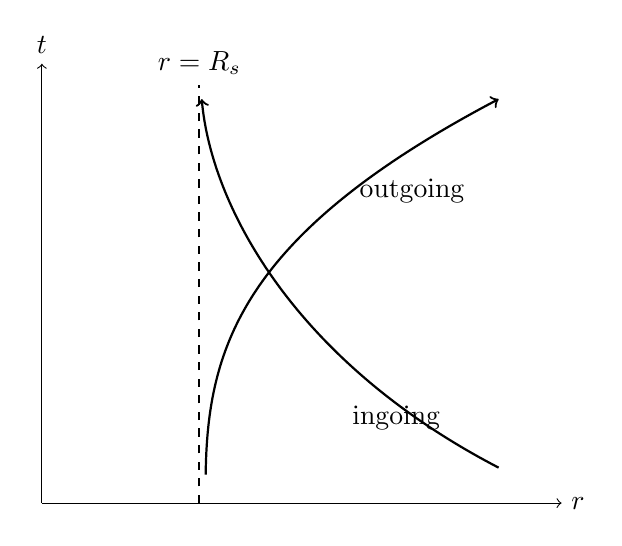
\begin{tikzpicture}[x=1.0cm,y=0.9cm]
\draw[->] (0,0) -- (6.6,0) node[right] {$r$};
\draw[->] (0,0) -- (0,6.2) node[above] {$t$};
\draw[dashed,thick] (2.0,0) -- (2.0,5.9) node[above] {$r=R_s$};
\draw[thick,->] (2.08,.4) .. controls (2.10,2.2) and (2.55,3.8) .. (5.8,5.7);
\draw[thick,->] (5.8,.5) .. controls (3.2,2.0) and (2.15,4.2) .. (2.03,5.7);
\node[align=center] at (4.7,4.4) {outgoing};
\node[align=center] at (4.5,1.2) {ingoing};
\end{tikzpicture}
\caption{Versión depurada del esquema de la pizarra en tiempo coordenado. La aparente ralentización se refiere a \(t\) de Schwarzschild, no a una incapacidad local de la luz para propagarse a \(c\).}
\end{figure}

Dentro del horizonte, los conos de luz futuros se inclinan tanto hacia dentro que ambas ramas radiales dirigidas al futuro avanzan hacia valores decrecientes de \(r\). Ninguna señal que se origine allí puede escapar al exterior, y toda trayectoria causal futura alcanza la singularidad.

\begin{classroomqa}
\audiencequestion{Si la velocidad de la luz es invariante, ¿qué significa exactamente decir que la luz se ralentiza cerca del horizonte?\lecturetimestamp{00:31:44}}
\lecturerresponse{La cantidad mostrada es \(dr/dt\) en un sistema de coordenadas concreto. La velocidad numérica ya cambia al sustituir metros por centímetros; aquí, las calibraciones radial y temporal efectivas varían con la posición. La afirmación universal es que todo rayo de luz sigue una trayectoria nula, \(ds^2=0\).}
\end{classroomqa}
\editorialnote{Un observador local en caída libre mide que la luz en el vacío se propaga a \(c\); la velocidad coordenada de Schwarzschild que se anula en el horizonte no es una magnitud observable localmente.}

\begin{classroomqa}
\audiencequestion{¿Se cumple la misma afirmación sobre la velocidad nula con independencia del medio material por el que se propaga la luz?\lecturetimestamp{00:33:24}}
\lecturerresponse{No. El reconocimiento disponible no conserva una explicación más extensa de esta respuesta.}
\end{classroomqa}
\editorialnote{La afirmación sobre la velocidad nula se refiere a la propagación en el espacio-tiempo vacío. Las interacciones con la materia pueden dar a un paquete de ondas una velocidad efectiva menor; eso es una propiedad del medio, no un cambio en la velocidad causal local \(c\).}

\begin{classroomqa}
\audiencequestion{¿Cómo se ve un rayo de luz entrante en el mismo diagrama \(t\)-\(r\)?\lecturetimestamp{00:33:32}}
\lecturerresponse{Es la rama que parece recorrer el camino inverso: desde valores grandes de \(r\) se curva hacia el horizonte y se aproxima a él asintóticamente. Tarda un tiempo coordenado infinito \(t\) en llegar.}
\end{classroomqa}
\editorialnote{Un observador en caída libre alcanza y cruza el horizonte en un tiempo propio finito; solo diverge \(t\) de Schwarzschild.}

\section{Por qué la evaporación plantea un problema}

El horizonte merece estudiarse mucho más: cómo se forma, qué ve un observador en caída libre y si ocurre allí algo inusual a nivel local. Susskind aplaza esas preguntas y pasa a la mecánica cuántica. Desde el exterior, la materia y toda la información que la distingue quedan cada vez más comprimidas cerca del horizonte y dejan de estar disponibles. Eso por sí solo no tiene por qué destruir la información; quizá solo la oculte.

El resultado de Hawking vuelve apremiante la cuestión. Desde el punto de vista clásico, un agujero negro en equilibrio parece el objeto más anodino imaginable: esférico, oscuro e incapaz de enviar un mensaje. Pero ``negro'' tiene dos sentidos. Puede significar que no emite nada o que emite radiación térmica de cuerpo negro. Un agujero negro cuántico es negro en el segundo sentido. Tiene temperatura, brilla y pierde energía. Como
\begin{equation}
E=Mc^2,
\qquad
R_s=\frac{2GM}{c^2},
\end{equation}
la radiación reduce tanto su masa como el radio de su horizonte. Si la evaporación acaba eliminando el agujero, ¿qué ocurre con la información que parecía permanecer en el horizonte? Podría destruirse, quedar atrapada en un remanente diminuto o codificarse en la radiación saliente. La tensión entre esas posibilidades constituye el problema de la información, y más adelante la teoría de cuerdas ayudará a precisar su resolución.

Esta noche no se intenta calcular campos cuánticos en el espacio-tiempo curvo. En su lugar, Susskind sigue el camino más sencillo de Bekenstein: primero entender la entropía como información y luego calcular cuánta información puede ocultar un agujero negro.

\section{Información presente pero oculta}

Imaginemos que dividimos una caja en celdas lo bastante pequeñas como para que cada una esté ocupada o vacía. Una cadena binaria---una respuesta por celda---distingue esa configuración de cualquier otra configuración permitida. Para describir materia más realista hay que preguntar por las especies de partículas y otros grados de libertad, pero el principio no cambia: la información se mide por el número mínimo de respuestas afirmativas--negativas necesarias para especificar el estado.

\begin{classroomqa}
\audiencequestion{¿Es esto solo una descripción de un sistema estático?\lecturetimestamp{00:45:49}}
\lecturerresponse{Es una descripción instantánea, correspondiente a un momento dado. La dinámica lleva después ese estado a otro estado.}
\end{classroomqa}

El siguiente principio es más profundo: la evolución de un sistema cerrado no fusiona dos estados microscópicos distintos en uno solo. Si dos configuraciones difieren ahora, sus configuraciones evolucionadas siguen siendo distinguibles en principio. La evolución hamiltoniana clásica es invertible y la evolución cuántica es unitaria.\editorialnote{Las ecuaciones efectivas disipativas solo pueden borrar distinciones porque se han omitido grados de libertad ambientales no observados; el estado completo del sistema cerrado las conserva.}

La bañera hace concreta la diferencia entre pérdida e inaccesibilidad. Dos corrientes de gotas podrían codificar dos textos distintos en código Morse. Cuando el agua se calma, las dos bañeras parecen iguales. Las ondas visibles han desaparecido, pero una medición microscópica completa aún encontraría configuraciones moleculares distintas. El mensaje se ha dispersado entre grados de libertad demasiado pequeños y demasiado numerosos para seguirles la pista.

La entropía es esa información oculta. Respecto de las preguntas macroscópicas que podemos plantear---temperatura, energía total, composición, nivel del agua---siguen siendo posibles muchas distinciones microscópicas, aunque no podamos acceder a ellas. En el lenguaje de la clase, basado en contar bits,
\begin{equation}
S=\hbox{number of hidden bits}.
\end{equation}
La fórmula estadística precisa es \(S=k_B\ln\Omega\), pero para el argumento sobre los agujeros negros basta con la definición cualitativa.

\section{La temperatura como coste de ocultar un bit}

La temperatura es fácil de medir y sorprendentemente indirecta de definir. Susskind toma la entropía y la energía como conceptos primitivos. Supongamos que se restablece un bit de computadora a un valor estándar. El dispositivo físico permanece, pero la computadora pierde la distinción entre sus estados anteriores, cero y uno. Esa distinción no puede desaparecer del mundo completo; se transfiere a grados de libertad microscópicos del entorno, que se calienta un poco. Este es el principio de Landauer.

Si una unidad de entropía equivale a un bit y la temperatura se mide en unidades de energía, la clase escribe
\begin{align}
\Delta S&=1,\\
\Delta E&=T\,\Delta S,\\
dE&=T\,dS.
\label{eq:first-law}
\end{align}

\begin{figure}[htbp]
\centering
\includegraphics[width=0.84\textwidth]{lecture_02_figure_04.png}
\caption{Termodinámica de la información en la pizarra: \(S\) es la entropía, un bit oculto tiene \(\Delta S=1\) y su coste energético mínimo se escribe \(\Delta E=T\Delta S\).}
\lectureframe{00:58:40.000}
\end{figure}

\editorialnote{En unidades convencionales, el coste de borrar reversiblemente un bit binario es \(k_BT\ln2\). La ecuación~\eqref{eq:first-law} usa \(k_B=1\) y toma la unidad de entropía de la clase como un bit, omitiendo el factor \(\ln2\) correspondiente. Estas convenciones no afectan el argumento de escala que sigue.}

Una estimación propuesta por alguien del público sitúa cerca de \(10^{-15}\) grados el aumento mínimo de temperatura del agua de un vaso al borrar aproximadamente \(100\) gigabytes. Susskind acepta la idea, no la cifra exacta: a temperatura ambiente, la energía mínima asociada a un bit es extraordinariamente pequeña, y las computadoras reales disipan mucho más porque el borrado no se realiza reversiblemente.

\begin{classroomqa}
\audiencequestion{¿El ejemplo del disco duro es solo una analogía, o el calentamiento al borrar información es una ley física real?\lecturetimestamp{01:00:02}}
\lecturerresponse{Es una restricción física real: la regla de Landauer. Al restablecer una celda de memoria se elimina de la computadora la distinción anterior, así que esa información debe trasladarse al entorno. Las operaciones ordinarias son mucho menos eficientes que el mínimo ideal porque también accionan circuitos, mueven cargas y generan calor no relacionado.}
\end{classroomqa}

\begin{classroomqa}
\audiencequestion{¿Ocultar un bit cuesta más energía a una temperatura más alta?\lecturetimestamp{01:02:07}}
\lecturerresponse{Sí. La relación \(dE=T\,dS\) lo expresa exactamente: para la misma transferencia de entropía, un baño térmico más caliente requiere una transferencia de energía mayor. También se puede considerar esta relación entre energía y bit oculto como una definición de la temperatura.}
\end{classroomqa}

\begin{classroomqa}
\audiencequestion{Si se sobrescribe un bit almacenado previamente, ¿se ha perdido esa información anterior?\lecturetimestamp{01:02:43}}
\lecturerresponse{Ha salido de la computadora, pero no ha desaparecido del sistema físico cerrado. La distinción sobrescrita se ha dispersado en el entorno, donde contribuye a la información inaccesible y, por tanto, a la entropía.}
\end{classroomqa}

La identificación de la entropía termodinámica con la información microscópica que falta se remonta a Boltzmann; Shannon aportó el lenguaje correspondiente de la teoría de la información en el siglo XX. Susskind comenta que esta explicación estaba extrañamente ausente de los cursos de termodinámica que él y algunos asistentes habían cursado en los años 1950. La informática hizo más difícil pasar por alto esta conexión, pero no originó su contenido físico.

\section{Introducir un bit en un agujero negro}

Ahora podemos construir conceptualmente un agujero negro, bit a bit, igual que se puede llenar una bañera, gota a gota. La pregunta es diferencial: cuando se oculta un bit más, ¿cuánto crece el horizonte? Empecemos con un agujero de masa \(M\) y radio \(R_s\), y enviemos después el objeto más sencillo cuya única distinción recuperable es si fue absorbido.

\begin{classroomqa}
\audiencequestion{¿No necesita la información un tiempo coordenado infinito para entrar en el agujero?\lecturetimestamp{01:08:07}}
\lecturerresponse{Se comprime exponencialmente cerca del horizonte y deja de estar disponible para el exterior en un tiempo práctico breve, aunque el tiempo coordenado de Schwarzschild asigne un valor infinito al cruce efectivo. Para llevar las cuentas desde el exterior, por tanto, puede tratarse como información almacenada en el horizonte.}
\end{classroomqa}

Un fotón es una opción natural, pero un fotón genérico transporta más de un bit. Su polarización puede codificar una elección binaria. Un punto de llegada muy localizado aporta muchas preguntas adicionales de respuesta sí--o no: hemisferio superior o inferior, mitad izquierda o derecha, y así sucesivamente. La mecánica cuántica limita la localización a una escala del orden de una longitud de onda; por eso, para suprimir la información posicional, hay que usar la longitud de onda más larga que el agujero todavía pueda absorber.

\begin{classroomqa}
\audiencequestion{¿Existe de verdad una longitud de onda máxima por encima de la cual el fotón no puede entrar?\lecturetimestamp{01:12:15}}
\lecturerresponse{Sí. Una onda mucho mayor que el agujero se dispersa principalmente, en vez de ser absorbida. La opción marginal útil es una longitud de onda comparable al radio del horizonte: lo bastante larga para borrar el punto de entrada, pero lo bastante corta para tener una probabilidad de absorción apreciable.}
\end{classroomqa}

\begin{classroomqa}
\audiencequestion{¿La dirección desde la que llega el fotón también aporta información?\lecturetimestamp{01:13:28}}
\lecturerresponse{Para una longitud de onda del orden del tamaño del horizonte, el campo varía tan lentamente a lo largo del agujero que la dirección de llegada no puede determinarse con gran precisión. Por eso, el límite de longitud de onda larga se aproxima a un único dato de respuesta sí--o no, en vez de a un impacto localizado con precisión.}
\end{classroomqa}

Así pues, tomemos, en orden de magnitud,
\begin{equation}
\lambda\sim R_s=\frac{2GM}{c^2}.
\label{eq:one-bit-wave}
\end{equation}
La cinemática del fotón da
\begin{equation}
E=cp,
\qquad
p=\hbar k=\frac{h}{\lambda},
\qquad
\Delta E\sim\frac{\hbar c}{R_s}.
\label{eq:one-bit-energy}
\end{equation}
Aquí \(k=2\pi/\lambda\) y \(h=2\pi\hbar\). La clase omite deliberadamente el factor \(2\pi\), así como los factores de absorción de orden unidad.

\begin{classroomqa}
\audiencequestion{¿Debe escribirse el momento como \(\hbar/\lambda\) o como \(h/\lambda\)?\lecturetimestamp{01:16:00}}
\lecturerresponse{Si \(\lambda\) es la longitud de onda ordinaria, la relación exacta es \(p=h/\lambda=2\pi\hbar/\lambda\); si usamos el número de onda \(k=2\pi/\lambda\), es \(p=\hbar k\). La estimación presente solo conserva la escala, así que se descarta intencionadamente el factor \(2\pi\).}
\end{classroomqa}

El coste energético de ocultar un bit viene dado por la escala de temperatura. Por tanto, las ecuaciones~\eqref{eq:one-bit-wave} y~\eqref{eq:one-bit-energy} dan
\begin{equation}
k_BT_H\sim\frac{\hbar c}{R_s}
\sim\frac{\hbar c^3}{GM}.
\end{equation}
El resultado exacto de Hawking es
\begin{equation}
k_BT_H=\frac{\hbar c^3}{8\pi GM}.
\end{equation}
El argumento elemental obtiene la dependencia respecto de \(M,G,c,\hbar\), pero no el coeficiente.

\section{Un bit ocupa una celda de escala de Planck}

El mismo fotón nos indica cómo crece el horizonte. Su energía cambia la masa en
\begin{equation}
\Delta M=\frac{\Delta E}{c^2}
\sim\frac{\hbar}{cR_s}.
\end{equation}
Como \(R_s=2GM/c^2\),
\begin{equation}
\Delta R_s=\frac{2G}{c^2}\Delta M
\sim\frac{G\hbar}{c^3R_s},
\end{equation}
donde de nuevo se han omitido todos los factores de orden unidad. Al multiplicar por \(R_s\),
\begin{equation}
R_s\Delta R_s\sim\frac{G\hbar}{c^3}.
\end{equation}
Como \(A=4\pi R_s^2\), su diferencial es \(dA=8\pi R_s\,dR_s\). Por tanto,
\begin{equation}
\Delta A\sim\frac{G\hbar}{c^3}=\ell_P^2,
\qquad
\ell_P=\sqrt{\frac{G\hbar}{c^3}}.
\label{eq:planck-patch}
\end{equation}

\begin{figure}[htbp]
\centering
\includegraphics[width=0.84\textwidth]{lecture_02_figure_05.png}
\caption{El argumento de escala completo en la pizarra: la energía de un bit, \(\Delta E\sim\hbar c/R_s\), conduce a un incremento del radio al cuadrado y, por tanto, del área, del orden de \(G\hbar/c^3\).}
\lectureframe{01:22:40.000}
\end{figure}

Durante el cálculo en directo, se vuelven a introducir a mitad de camino los factores de \(c\) y alguien del público detecta que falta \(c^{-2}\) en el radio de Schwarzschild. Esa corrección es precisamente la que produce el factor \(c^{-3}\) en la ecuación~\eqref{eq:planck-patch}.

\begin{classroomqa}
\audiencequestion{Al restituir \(c\) solo en una parte del cálculo, ¿se perdieron dos potencias?\lecturetimestamp{01:21:18}}
\lecturerresponse{Sí. La relación dimensional es \(R_s=2GM/c^2\), no simplemente \(2GM\). Al restituir ese factor, el área escala como \(G\hbar/c^3\).}
\end{classroomqa}

Usando \(G\simeq6.7\times10^{-11}\,\mathrm{m^3\,kg^{-1}\,s^{-2}}\), \(\hbar\simeq1.05\times10^{-34}\,\mathrm{J\,s}\) y \(c^3\simeq2.7\times10^{25}\,\mathrm{m^3\,s^{-3}}\),
\begin{equation}
\ell_P^2\simeq2.6\times10^{-70}\,\mathrm{m^2},
\qquad
\ell_P\simeq1.6\times10^{-35}\,\mathrm{m}.
\end{equation}
Las potencias mencionadas oralmente en la clase varían mientras se hace la estimación en la pizarra; la conclusión física se mantiene. Esta escala queda muy por debajo de la resolución experimental directa.

La imagen memorable es la de bits impenetrables, con los codos afilados, que se acumulan en el horizonte y se empujan unos a otros. Cada bit nuevo ocupa aproximadamente una celda de área de Planck. Es una metáfora para llevar la cuenta del área, no una afirmación de que el horizonte esté formado por baldosas cuadradas literales.

\begin{classroomqa}
\audiencequestion{Si el primer fotón sigue acercándose cuando otro fotón agranda el horizonte, ¿no queda el primero dentro del nuevo horizonte?\lecturetimestamp{01:26:39}}
\lecturerresponse{El sencillo panorama estático no basta para resolver esa pregunta con precisión. El horizonte de sucesos en un espacio-tiempo dinámico debe definirse globalmente, y su posición cambia a medida que llega materia. En la descripción exterior que usamos aquí, la información sigue asociada al horizonte en expansión. Dejamos para más adelante una definición cuidadosa de ese horizonte.}
\end{classroomqa}

\begin{classroomqa}
\audiencequestion{¿Se plantearía el mismo problema al añadir una masa enorme, por ejemplo, cuando chocan dos agujeros negros?\lecturetimestamp{01:27:03}}
\lecturerresponse{Sí; en ese caso es imposible ignorar el carácter dinámico. La clase aplaza el estudio completo de la geometría de la fusión hasta haber definido el horizonte con más cuidado.}
\end{classroomqa}

\begin{classroomqa}
\audiencequestion{¿Se define el área de Planck solo en una celda plana, y no sobre un horizonte esférico?\lecturetimestamp{01:27:30}}
\lecturerresponse{Es una escala de área sobre la superficie esférica; no exige que el horizonte sea plano. La distinción entre plano y esférico no es relevante para este recuento.}
\end{classroomqa}
\editorialnote{Cuando el radio de curvatura del horizonte es enorme en comparación con \(\ell_P\), cada entorno de tamaño de Planck es casi plano localmente.}

Para un agujero de ocho kilómetros de diámetro, el fotón marginal correspondiente es una onda de radio larga, de una escala aproximadamente igual. Una analogía planteada por alguien del público compara el incremento del área, independiente del tamaño, con añadir la misma circunferencia extra a una cuerda enrollada alrededor de una pelota de baloncesto o de la Tierra: en ambos casos, la separación radial que crea una circunferencia añadida fija es la misma. Las geometrías exactas difieren, pero ambos ejemplos aíslan un cambio independiente del tamaño original del objeto.

\section{La ley del área}

Añadir un bit cada vez modifica el área del horizonte en una cantidad microscópica universal. Por tanto, el número de bits que se pueden ocultar debe ser proporcional a \(A/\ell_P^2\), no al volumen. Bekenstein dedujo la proporcionalidad; el cálculo de Hawking fijó su coeficiente:
\begin{equation}
S_{\mathrm{BH}}=\frac{k_B A c^3}{4G\hbar}
=\frac{k_B A}{4\ell_P^2}.
\label{eq:bh-entropy}
\end{equation}
Si la entropía se cuenta en bits binarios en vez de en unidades termodinámicas, hay que dividir \(S_{\mathrm{BH}}/k_B\) por \(\ln2\).

\begin{figure}[htbp]
\centering
\includegraphics[width=0.84\textwidth]{lecture_02_figure_06.png}
\caption{Fórmula final en la pizarra, incluido el factor de Hawking \(1/4\): \(S\propto Ac^3/(4G\hbar)\) en las unidades de entropía de la clase.}
\lectureframe{01:31:02.000}
\end{figure}

Por tanto, los agujeros negros tienen mucha más entropía que los sistemas ordinarios de tamaño comparable. Aun así, el resultado es menor de lo que sugeriría un recuento ingenuo basado en el volumen. La información independiente está limitada por una magnitud superficial. Esta inversión---una región gravitante tridimensional descrita mediante información que escala como una frontera bidimensional---es la semilla del principio holográfico.

\begin{classroomqa}
\audiencequestion{¿De dónde viene el factor \(1/4\) de la fórmula de la entropía?\lecturetimestamp{01:30:30}}
\lecturerresponse{El argumento de Bekenstein fijó la dependencia respecto del área y las constantes fundamentales, pero dejó indeterminado el coeficiente; sus estimaciones dieron posibilidades como los logaritmos de dos. El cálculo de Hawking con campos cuánticos fijó el coeficiente exactamente en \(1/4\).}
\end{classroomqa}

La posición de \(\hbar\) contiene la sorpresa final. Cabría esperar que una entropía cuántica fuera proporcional a \(\hbar\) y se anulara en el límite clásico. En cambio, \(\hbar\) está en el denominador. Cuando \(\hbar\to0\), una onda puede transportar información arbitrariamente precisa con un coste energético arbitrariamente pequeño, por lo que la capacidad de entropía diverge. La cuantización no añade una pequeña entropía a un agujero que, por lo demás, sería clásico; impide que la capacidad de información sea infinita.

\begin{classroomqa}
\audiencequestion{¿Por qué \(\hbar\), que tiene unidades de momento angular, también determina la relación entre el momento ordinario y la longitud de onda?\lecturetimestamp{01:33:23}}
\lecturerresponse{\(\hbar\) tiene unidades de acción, equivalentes a momento por distancia. Como \(p\lambda\) tiene las mismas unidades, la relación cuántica puede ser \(p\sim\hbar/\lambda\), salvo por la convención de \(2\pi\). El momento angular \(\mathbf r\times\mathbf p\) tiene las mismas dimensiones por la misma razón.}
\end{classroomqa}

La clase termina aquí, no porque se haya agotado el tema, sino porque este es el límite adecuado. La geometría nos ha explicado por qué el horizonte oculta información; la termodinámica nos ha enseñado a contarla, y la mecánica cuántica ha proporcionado un área finita por bit. La siguiente pregunta ya no es si un agujero negro tiene estados microscópicos, sino cómo esos estados codifican y, finalmente, devuelven lo que cayó en él.
